

\section{Experiments}
\label{sec:exp}


\begin{table*}[h]
\vspace{-0.4cm}
\begin{center}
% \scriptsize
\scalebox{0.8}
{
\begin{tabular}{c|ccccccc} \hline
Datasets       & ETTh1$\&$ETTh2       & ETTm1 $\&$ETTm2        & Traffic     & Electricity  & Exchange-Rate & Weather      & ILI      \\ \hline
Variates       & 7          & 7            & 862         & 321          & 8             & 21          & 7      \\
Timesteps      & 17,420     & 69,680       & 17,544      & 26,304       & 7,588         & 52,696       & 966     \\
Granularity    & 1hour      & 5min         & 1hour       & 1hour        & 1day          & 10min        & 1week    \\ \hline
\end{tabular}}
\end{center}
\vspace{-0.5cm}
\caption{The statistics of the nine popular datasets for the LTSF problem.}
\label{tab:datasets}
\vspace{-0.2cm}
\end{table*}


\begin{table*}[t!]
\centering
%\scriptsize
\scalebox{0.7}{
\begin{tabular}{c|c|c|cccccc||cccccccccc|cc}
\hline
\multicolumn{2}{c|}{Methods}&{IMP.}&\multicolumn{2}{c|}{Linear*}&\multicolumn{2}{c|}{NLinear*}&\multicolumn{2}{c||}{DLinear*} &\multicolumn{2}{c|}{FEDformer}&\multicolumn{2}{c|}{Autoformer}&\multicolumn{2}{c|}{Informer}&\multicolumn{2}{c|}{Pyraformer*}&\multicolumn{2}{c|}{LogTrans}&\multicolumn{2}{c}{\emph{Repeat}*}\\
\hline
\multicolumn{2}{c|}{Metric} & MSE & MSE  & MAE& MSE  & MAE& MSE  & MAE& MSE  & MAE& MSE  & MAE& MSE  & MAE& MSE & MAE& MSE & MAE& MSE & MAE\\
\hline
\multirow{4}{*}{\rotatebox{90}{Electricity}}
&96&27.40\%&\textbf{0.140} & \textbf{0.237} & 0.141 & \textbf{0.237} & \textbf{0.140} & \textbf{0.237} & {\underline{0.193}} & \underline{0.308} & 0.201 & 0.317 & 0.274 & 0.368 & 0.386 & 0.449 & 0.258 & 0.357 & 1.588 & 0.946 \\
&192&23.88\%&\textbf{0.153} & 0.250 & 0.154 & \textbf{0.248} & \textbf{0.153} & {0.249} & \underline{0.201} & \underline{0.315} & 0.222 & 0.334 & 0.296 & 0.386 & 0.386 & 0.443 & 0.266 & 0.368 & 1.595 & 0.950 \\
&336&21.02\%&\textbf{0.169} & 0.268 & 0.171 & \textbf{0.265} & \textbf{0.169} & {0.267} & \underline{0.214} & \underline{0.329} & 0.231 & 0.338 & 0.300 & 0.394 & 0.378 & 0.443 & 0.280 & 0.380 & 1.617 & 0.961 \\
&720&17.47\%&\textbf{0.203} & {0.301} & {0.210} & \textbf{0.297} & \textbf{0.203} & {0.301} & \underline{0.246} & \underline{0.355} & 0.254 & 0.361 & 0.373 & 0.439 & 0.376 & 0.445 & 0.283 & 0.376 & 1.647 & 0.975 \\
\hline
\multirow{4}{*}{\rotatebox{90}{Exchange}}
&96&45.27\%&0.082 & 0.207 & 0.089 & 0.208 & \textbf{0.081} & {0.203} & \underline{0.148} & \underline{0.278} & 0.197 & 0.323 & 0.847 & 0.752 & 0.376 & 1.105 & 0.968 & 0.812 & {\textbf{0.081}} & {\textbf{0.196}} \\
&192&42.06\%&{0.167} & 0.304 & 0.180 & 0.300 & \textbf{0.157} & {0.293} & \underline{0.271} & \underline{0.380} & 0.300 & 0.369 & 1.204 & 0.895 & 1.748 & 1.151 & 1.040 & 0.851 & {0.167} & {\textbf{0.289}} \\
&336&33.69\%&0.328 & 0.432 & 0.331 & 0.415 & \textbf{0.305} & {0.414} & \underline{0.460} & \underline{0.500} & 0.509 & 0.524 & 1.672 & 1.036 & 1.874 & 1.172 & 1.659 & 1.081 & \textbf{0.305} & \textbf{0.396} \\
&720&46.19\%&0.964 & 0.750 & 1.033 & 0.780 & \textbf{0.643} & \textbf{0.601} & \underline{1.195} & \underline{0.841} & 1.447 & 0.941 & 2.478 & 1.310 & 1.943 & 1.206 & 1.941 & 1.127 & {0.823} & {0.681} \\
\hline
\multirow{4}{*}{\rotatebox{90}{Traffic}}
&96&30.15\%&\textbf{0.410} & {0.282} & \textbf{0.410} & \textbf{0.279} & \textbf{0.410} & {0.282} & {\underline{0.587}} & {\underline{0.366}} & {{0.613}} & 0.388 & 0.719 & 0.391 & 2.085 & 0.468 & 0.684 & {{0.384}} & 2.723 & 1.079 \\
&192&29.96\%&\textbf{0.423} & {0.287} & \textbf{0.423} & \textbf{0.284} & \textbf{0.423} & {0.287} & \underline{0.604} & {\underline{0.373}} & 0.616 & 0.382 & 0.696 & 0.379 & 0.867 & 0.467 & 0.685 & 0.390 & 2.756 & 1.087 \\
&336&29.95\%&{0.436} & {0.295} & \textbf{0.435} & \textbf{0.290} & 0.436 & 0.296 & \underline{0.621} & {0.383} & {0.622} & {\underline{0.337}} & 0.777 & 0.420 & 0.869 & 0.469 & 0.734 & 0.408 & 2.791 & 1.095 \\
&720&25.87\%&{0.466} & {0.315} & \textbf{0.464} & \textbf{0.307} & {0.466} & {0.315} & {\underline{0.626}} & {\underline{0.382}} & 0.660 & 0.408 & 0.864 & 0.472 & 0.881 & 0.473 & 0.717 & 0.396 & 2.811 & 1.097 \\
\hline
\multirow{4}{*}{\rotatebox{90}{Weather}}
&96&18.89\%&\textbf{0.176} & {0.236} & 0.182 & \textbf{0.232} & \textbf{0.176} & 0.237 & \underline{0.217} & \underline{0.296} & 0.266 & 0.336 & 0.300 & 0.384 & 0.896 & 0.556 & 0.458 & 0.490 & 0.259 & {{0.254}} \\
&192&21.01\%&\textbf{0.218} & {0.276} & 0.225 & \textbf{0.269} & 0.220 & 0.282 &\underline{0.276} & \underline{0.336} & 0.307 & 0.367 & 0.598 & 0.544 & 0.622 & 0.624 & 0.658 & 0.589 & 0.309 & {{0.292}} \\
&336&22.71\%&\textbf{0.262} & {0.312} & 0.271 & \textbf{0.301} & 0.265 & 0.319 & \underline{0.339} & \underline{0.380} & 0.359 & 0.395 & 0.578 & 0.523 & 0.739 & 0.753 & 0.797 & 0.652 & 0.377 & 0.338 \\
&720&19.85\%&0.326 & 0.365 & 0.338 & \textbf{0.348} & \textbf{0.323} & {0.362} & \underline{0.403} & \underline{0.428} & 0.419 & 0.428 & 1.059 & 0.741 & 1.004 & 0.934 & 0.869 & 0.675 & 0.465 & 0.394 \\
\hline
\multirow{4}{*}{\rotatebox{90}{ILI}}
&24&47.86\%&{1.947} & {0.985} & \textbf{1.683} & \textbf{0.858} & 2.215 & 1.081 & \underline{3.228} & \underline{1.260} & 3.483 & 1.287 & 5.764 & 1.677 & 1.420 & 2.012 & 4.480 & 1.444 & 6.587 & 1.701 \\
&36&36.43\%&2.182 & 1.036 & \textbf{1.703} & \textbf{0.859} & {1.963} & {0.963} & {\underline{2.679}} & {\underline{1.080}} & 3.103 & 1.148 & 4.755 & 1.467 & 7.394 & 2.031 & 4.799 & 1.467 & 7.130 & 1.884 \\
&48&34.43\%&2.256 & 1.060 & \textbf{1.719} & \textbf{0.884} & {2.130} & {1.024} & \underline{2.622} & {\underline{1.078}} & 2.669 & 1.085 & 4.763 & 1.469 & 7.551 & 2.057 & 4.800 & 1.468 & 6.575 & 1.798 \\
&60&34.33\%&2.390 & 1.104 & \textbf{1.819} & \textbf{0.917} & {2.368} & {1.096} & {2.857} & {1.157} & {\underline{2.770}} & {\underline{1.125}} & 5.264 & 1.564 & 7.662 & 2.100 & 5.278 & 1.560 & 5.893 & 1.677 \\\hline
\multirow{4}{*}{\rotatebox{90}{ETTh1}}
 & 96 &0.80\% & {0.375} & { 0.397} & \textbf{0.374} & \textbf{0.394} & {  {0.375}} & { {0.399}}  & { \underline{0.376}} &{ \underline{0.419}}        & 0.449 & 0.459 & 0.865 & 0.713 & 0.664 & 0.612 & 0.878 & 0.740  &1.295	&0.713\\
 & 192  &3.57\% & 0.418 & 0.429 & {0.408} & \textbf{0.415} & { \textbf{0.405}} & {  {0.416}}  & \underline{  0.420} &{ \underline{0.448}}       & 0.500 & {0.482} & {1.008}  & 0.792 & 0.790 & 0.681 & 1.037 & 0.824  &1.325	&0.733\\
 & 336 &6.54\% & 0.479 & 0.476 & \textbf{0.429} & \textbf{0.427} & {  {0.439}} & {  {0.443}}   & { \underline{0.459}} &{ \underline{0.465}}       & 0.521 & 0.496 & 1.107 & 0.809 & 0.891 & 0.738 & 1.238 & 0.932  &1.323	&0.744\\
 & 720 &13.04\%& 0.624 & 0.592 & \textbf{0.440} & \textbf{0.453} & {  {0.472}} & {  {0.490}}        & { \underline{0.506}}    & { \underline{0.507}} &{ {0.514}} &{ {0.512}} & 1.181 & 0.865 & 0.963 & 0.782 & 1.135 & 0.852  &1.339	&0.756\\
\hline
\multirow{4}{*}{\rotatebox{90}{ETTh2}}
 & 96  & 19.94\%&  {0.288} &  {0.352}  & \textbf{0.277} & \textbf{0.338} & { {0.289}} & { {0.353}}          &{\underline{0.346}}    &{ \underline{0.388}}              & 0.358       & 0.397       & 3.755 & 1.525 & 0.645 & 0.597 & 2.116 & 1.197 &0.432	&0.422 \\
 & 192 & 19.81\%&  {0.377} &  {0.413}  &\textbf{0.344} & \textbf{0.381} & { {0.383}} & { {0.418}}                 & { \underline{0.429}} & { \underline{0.439}}    & 0.456       &{ {0.452}}       & 5.602 & 1.931 & 0.788 & 0.683 & 4.315 & 1.635 &0.534	&0.473 \\
 & 336 & 25.93\% & 0.452 & 0.461  & \textbf{0.357} & \textbf{0.400} & {  {0.448}} & {  {0.465}}                &{ \underline{0.496}}          &{ \underline{0.487}} & { {0.482}} & { {0.486}} & 4.721 & 1.835 & 0.907 & 0.747 & 1.124 & 1.604 &0.591	&0.508\\
 & 720 & 14.25\%& 0.698 & 0.595  & \textbf{0.394} & \textbf{0.436} & 0.605 & 0.551            & {  \underline{0.463}} & {  \underline{0.474} }&{ {0.515}}       &{ {0.511}}       & 3.647 & 1.625 & 0.963 & 0.783 & 3.188 & 1.540  &0.588	&0.517\\
\hline
\multirow{4}{*}{\rotatebox{90}{ETTm1}}
 & 96  & 21.10\% & 0.308 & 0.352  &  {0.306} &  {0.348} & { \textbf{0.299}} & { \textbf{0.343}} &{ \underline{0.379}}          &{ \underline{0.419} }        & 0.505       & 0.475       & 0.672 & 0.571 & 0.543 & 0.510 & 0.600 & 0.546  &1.214	&0.665\\
 & 192 & 21.36\% & {0.340} & {0.369}  & 0.349 & 0.375 & { \textbf{0.335}} & { \textbf{0.365}} &{ \underline{0.426}}          &{ \underline{0.441}}       & 0.553       & 0.496       & 0.795 & 0.669 & 0.557 & 0.537 & 0.837 & 0.700  &1.261	&0.690\\
 & 336 & 17.07\% & 0.376 & 0.393  & {0.375} & {0.388} & {\textbf {0.369}} & { \textbf{0.386}} &{ \underline{0.445}}          &{ \underline{0.459}}     & 0.621       & 0.537       & 1.212 & 0.871 & 0.754 & 0.655 & 1.124 & 0.832  &1.283	&0.707\\
 & 720 &21.73\% & 0.440 & 0.435  & {0.433} & {0.422} & { \textbf{0.425}} & { \textbf{0.421}} &{ \underline{0.543}}          &{ \underline{0.490} }     & 0.671       & 0.561       & 1.166 & 0.823 & 0.908 & 0.724 & 1.153 & 0.820  &1.319	&0.729\\
\hline
\multirow{4}{*}{\rotatebox{90}{ETTm2}} 
 & 96  & 17.73\% & 0.168 & 0.262  &\textbf{ 0.167} & \textbf{0.255} & { \textbf{0.167}} & { {0.260}} &{ \underline{0.203}}    &{\underline{0.287}}    & 0.255       & 0.339       & 0.365 & 0.453 & 0.435 & 0.507 & 0.768 & 0.642 & 0.266	& 0.328\\
 & 192 & 17.84\% & 0.232 & 0.308  & \textbf{0.221} & \textbf{0.293} & { {0.224}} & { {0.303}}      &{ \underline{0.269}}    &{\underline{0.328}}    & 0.281       & 0.340       & 0.533 & 0.563 & 0.730 & 0.673 & 0.989 & 0.757  & 0.340	& 0.371\\
 & 336 & 15.69\% & 0.320 & 0.373  & \textbf{0.274} & \textbf{0.327} & { {0.281}}    & { {0.342}}       & { \underline{0.325}} & { \underline{0.366}}  & 0.339       & 0.372       & 1.363 & 0.887 & 1.201 & 0.845 & 1.334 & 0.872  & 0.412	& 0.410\\
 & 720 & 12.58\% & 0.413 & 0.435 & \textbf{0.368} & \textbf{0.384} & { {0.397}}    & 0.421        & { \underline{0.421}} & { \underline{0.415}} & 0.433         & 0.432          & 3.379 & 1.338 & 3.625 & 1.451 & 3.048 & 1.328 & 0.521 &0.465\\
\hline
\end{tabular}
}
\begin{tablenotes} %添加此处
    \tiny
    {
    \item - Methods* are implemented by us; Other results are from FEDformer~\cite{zhou2022fedformer}.
    }
\end{tablenotes} %添加此处
\vspace{-0.2cm}
\caption{Multivariate long-term forecasting errors in terms of MSE and MAE, the lower the better. Among them, ILI dataset is with forecasting horizon $T \in \{24,36,48,60\}$. For the others, $T \in \{96,192,336,720\}$. \emph{Repeat} repeats the last value in the look-back window. The \textbf{best results} are highlighted in {\textbf{bold}} and the \underline{best results of Transformers} are highlighted with a { \underline{underline}}. Accordingly, IMP. is the best result of linear models compared to the results of Transformer-based solutions. }
\vspace{-0.5cm}
\label{tab:multi-benchmarks-ett}
\end{table*}


\begin{figure*}[h]	
	\subfigure[Electricity] %第一张子图
	{
		\begin{minipage}{5cm}
			\centering          %子图居中
			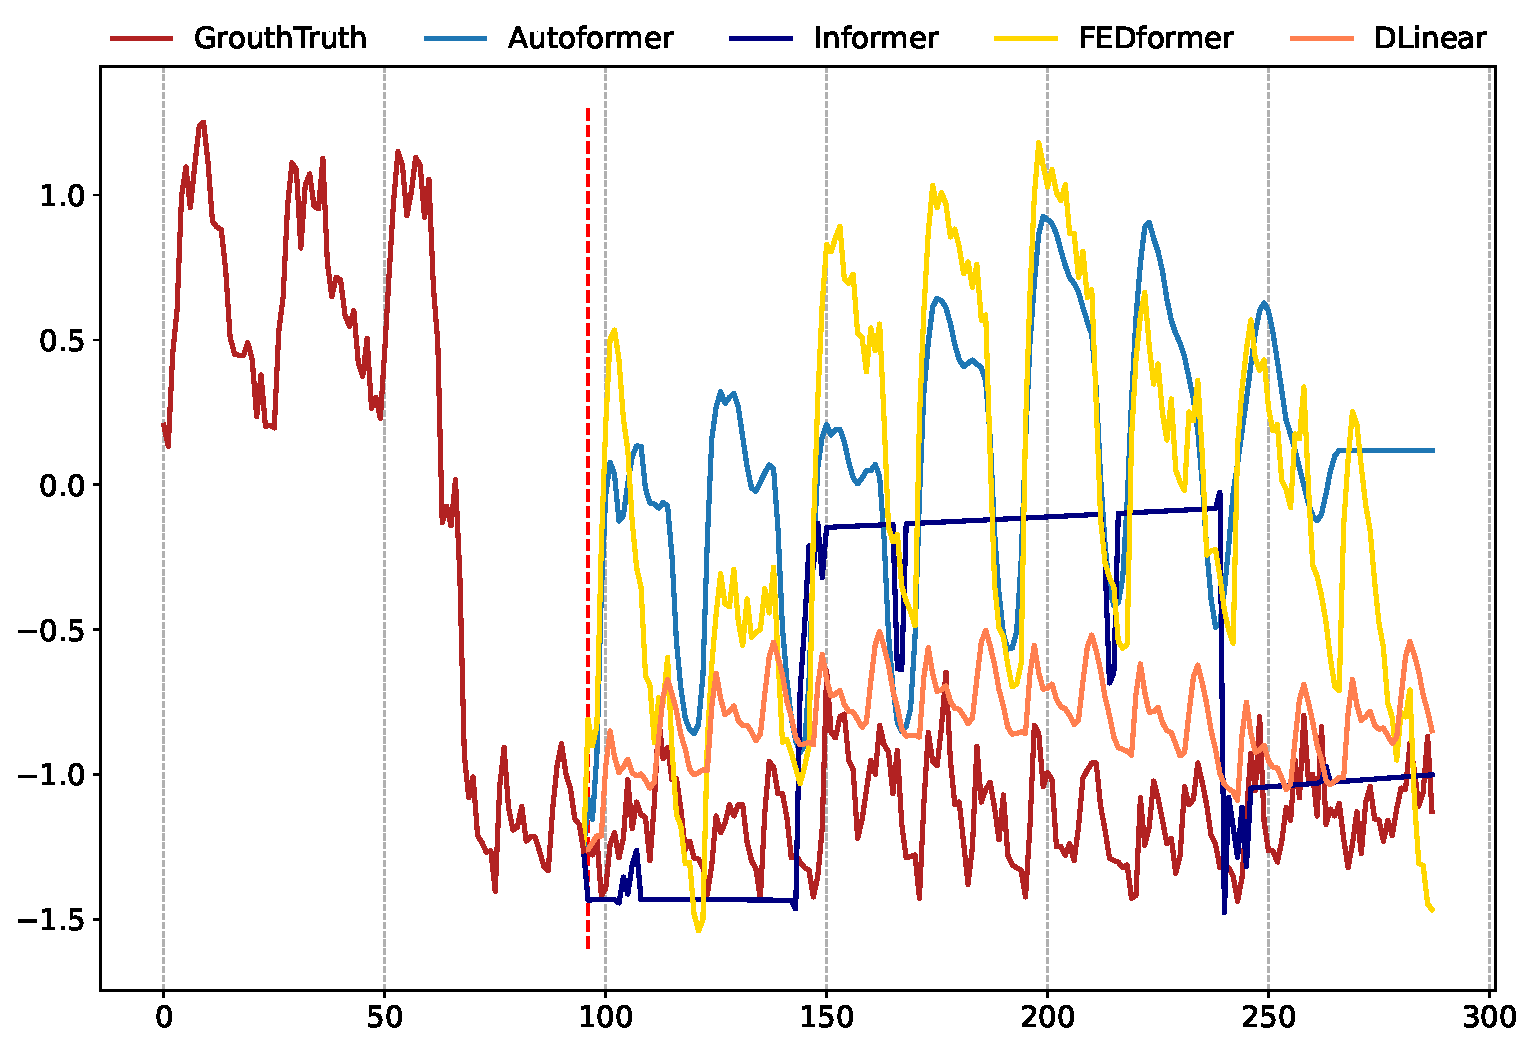
\includegraphics[scale=0.23]{img/ele_c36_s1951.pdf}   %以pic.jpg的0.4倍大小输出
		\end{minipage}
	}
	\hspace{0.55cm}
	\subfigure[Exchange-Rate] %第一张子图
	{
		\begin{minipage}{5cm}
			\centering          %子图居中
			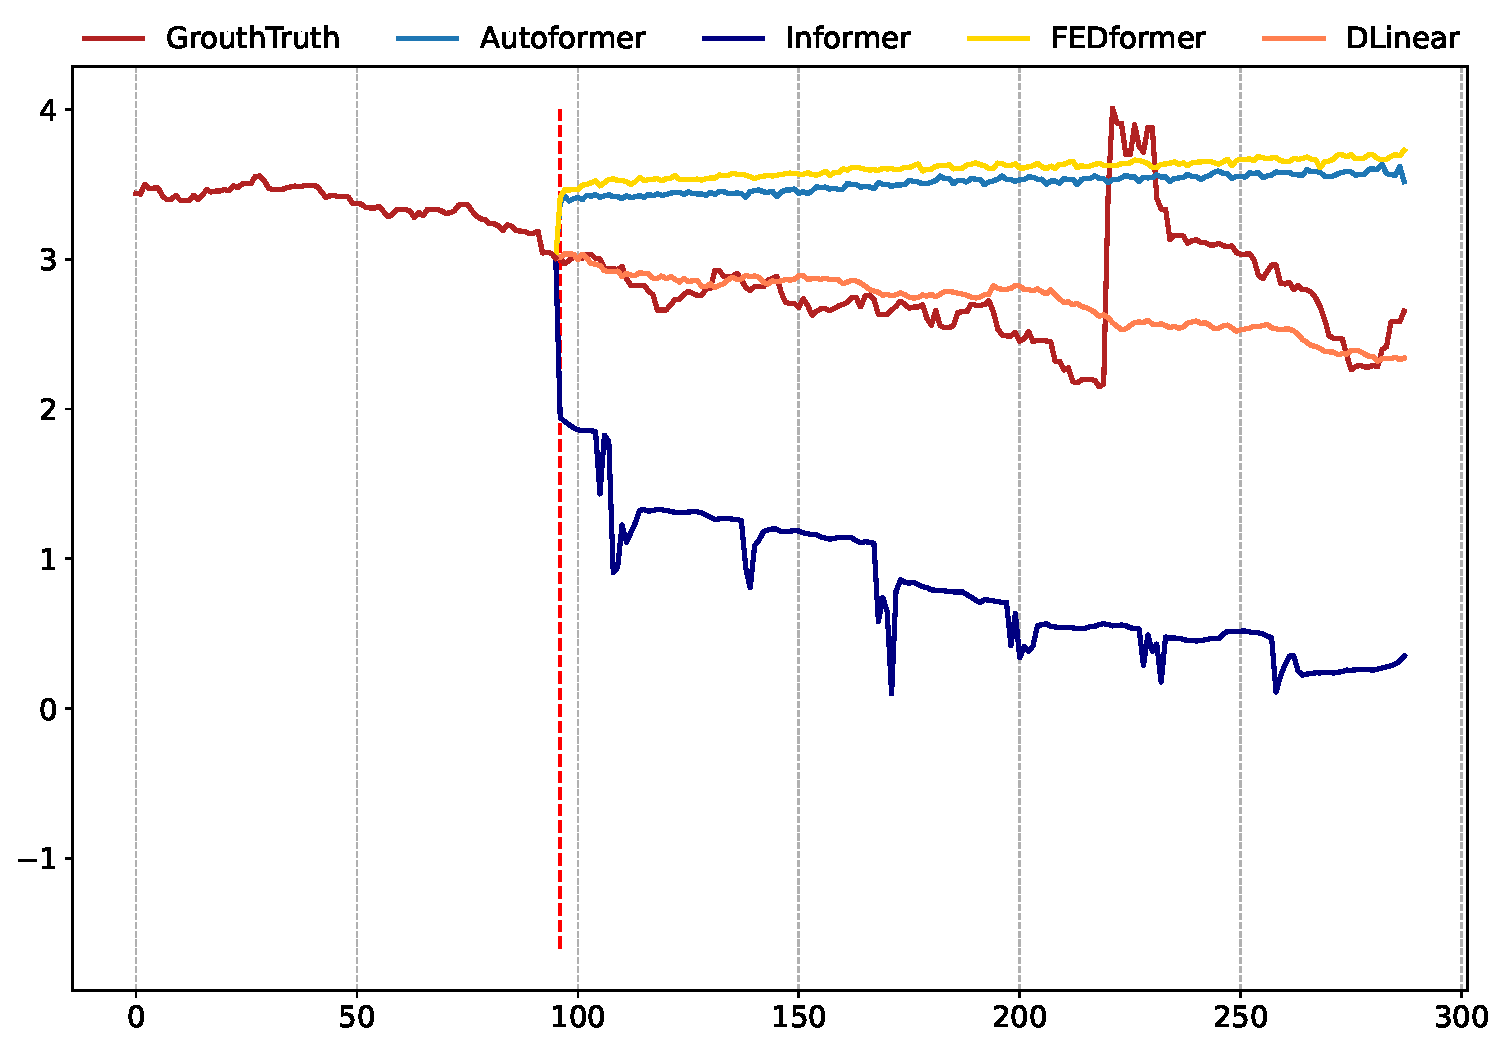
\includegraphics[scale=0.23]{img/exchange_c3_s676.pdf}   
		\end{minipage}
	}
	\hspace{0.45cm}
	\subfigure[ETTh2] %第二张子图
	{
		\begin{minipage}{5cm}
			\centering      %子图居中
			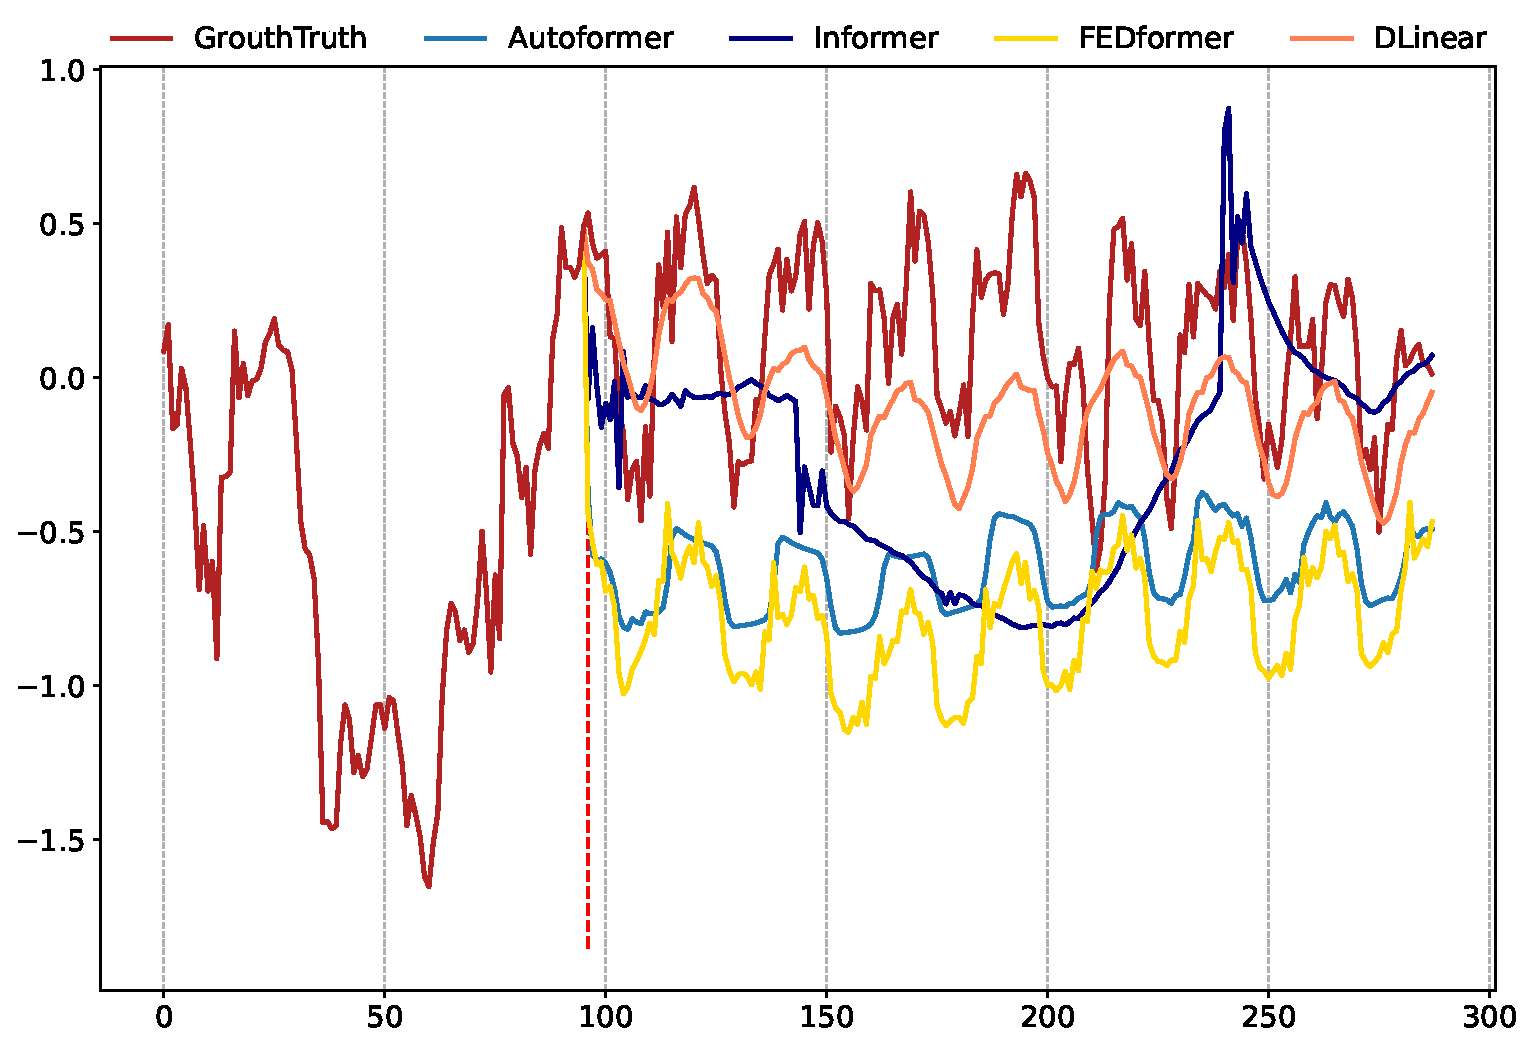
\includegraphics[scale=0.23]{img/etth2_good_c2_s1241.pdf}   
		\end{minipage}
	}
    \vspace{-0.3cm}
	\caption{Illustration of the long-term forecasting output (Y-axis) of five models with an input length $L$=96 and output length $T$=192 (X-axis) on Electricity, Exchange-Rate, and ETTh2, respectively.} % 
	\label{fig:visualize_prediction}  %图片引用标记
\vspace{-0.2cm}
\end{figure*}


\subsection{Experimental Settings}

\textbf{Dataset.} We conduct extensive experiments on nine widely-used real-world datasets, including ETT (Electricity Transformer Temperature)~\cite{informer} (ETTh1, ETTh2, ETTm1, ETTm2), Traffic, Electricity, Weather, ILI, Exchange-Rate~\cite{GuokunLai2017lstm}. All of them are multivariate time series. We leave \emph{data descriptions} in the Appendix.
%\vspace{-0.4cm}


\textbf{Evaluation metric.}
Following previous works~\cite{informer,xu2021autoformer,zhou2022fedformer}, we use Mean Squared Error (MSE) and Mean Absolute Error (MAE) as the core metrics to compare performance. 


\textbf{Compared methods.} We include five recent Transformer-based methods: FEDformer~\cite{zhou2022fedformer}, Autoformer~\cite{xu2021autoformer}, Informer~\cite{informer}, Pyraformer~\cite{liu2021pyraformer}, and LogTrans~\cite{li2019LogTrans}. 
Besides, we include a naive DMS method: Closest Repeat (\emph{Repeat}), which repeats the last value in the look-back window, as another simple baseline. Since there are two variants of FEDformer, we compare the one with better accuracy (FEDformer-f via Fourier transform). 
%More implementation details are in the Appendix.
% select two popular statistical methods: AutoARIMA~\cite{hyndman2008automatic} and GBRT~\cite{gbrt}, and 


\subsection{Comparison with Transformers}


\textbf{Quantitative results.} In Table~\ref{tab:multi-benchmarks-ett}, we extensively evaluate all mentioned Transformers on nine benchmarks, following the experimental setting of previous work~\cite{xu2021autoformer,zhou2022fedformer,informer}.
%
Surprisingly, the performance of \modelname surpasses the SOTA FEDformer in most cases by 20\% $\sim$ 50\% improvements on the \emph{multivariate forecasting}, where \modelname even does not model correlations among variates. For different time series benchmarks, \emph{NLinear} and \emph{DLinear} show the superiority to handle the distribution shift and trend-seasonality features.
%
%
We also provide results for \emph{univariate forecasting} of ETT datasets in the Appendix, where \modelname still consistently outperforms Transformer-based LTSF solutions by a large margin.
%

FEDformer achieves competitive forecasting accuracy on ETTh1. This because FEDformer employs classical time series analysis techniques such as frequency processing, which brings in time series inductive bias and benefits the ability of temporal feature extraction. 
%However, those complex modifications are still not as effective as the simple \modelname. 
In summary, these results reveal that existing complex Transformer-based LTSF solutions are not seemingly effective on the existing nine benchmarks while \modelname can be a powerful baseline. 



Another interesting observation is that even though the naive \emph{Repeat} method shows worse results when predicting long-term seasonal data (e.g., Electricity and Traffic), it surprisingly outperforms all Transformer-based methods on Exchange-Rate (around 45\%). 
%In fact, Transformers are hard to learn proper representation of time series  without periodicity.
This is mainly caused by the wrong prediction of trends in Transformer-based solutions, which may overfit toward sudden change noises in the training data, resulting in significant accuracy degradation (see Figure~\ref{fig:visualize_prediction}(b)). Instead, \emph{Repeat} does not have the bias.


\textbf{Qualitative results.}
As shown in Figure~\ref{fig:visualize_prediction}, we plot the prediction results on three selected time series datasets with Transformer-based solutions and \modelname: Electricity (Sequence 1951, Variate 36), Exchange-Rate (Sequence 676, Variate 3), and ETTh2 ( Sequence 1241, Variate 2), where these datasets have different temporal patterns. When the input length is 96 steps, and the output horizon is 336 steps, Transformers~\cite{informer,xu2021autoformer,zhou2022fedformer} fail to capture the scale and bias of the future data on Electricity and ETTh2. Moreover, they can hardly predict a proper trend on aperiodic data such as Exchange-Rate. These phenomena further indicate the inadequacy of existing Transformer-based solutions for the LTSF task.



\subsection{More Analyses on LTSF-Transformers}
\label{subsec:TransformerModelDesign}

\textbf{\emph{Can existing LTSF-Transformers extract temporal relations well from longer input sequences?}}
The size of the look-back window greatly impacts forecasting accuracy as it determines how much we can learn from historical data. Generally speaking, a powerful TSF model with a strong temporal relation extraction capability should be able to achieve better results with larger look-back window sizes.
%

To study the impact of input look-back window sizes, we conduct experiments with $L \in \{24, 48, 72, 96, 120, 144, 168, 192, 336, 504, 672, 720\}$ for long-term forecasting (T=720).
%
Figure~\ref{fig:lookBackWindows} demonstrates the MSE results on two datasets. 
%
Similar to the observations from previous studies~\cite{informer,wen2022transformers}, existing Transformer-based models' performance deteriorates or stays stable when the look-back window size increases. In contrast, the performances of all \modelname are significantly boosted with the increase of look-back window size. 
%That is, larger look-back window sizes generally harm the performance of existing Transformers. 
Thus, existing solutions tend to overfit temporal noises instead of extracting temporal information if given a longer sequence, and the input size 96 is exactly suitable for most Transformers.
%
Additionally, we provide more quantitative results in the Appendix, and our conclusion holds in almost all cases. 

\begin{figure}[h]	
    \hspace{-0.6cm}
	\subfigure[\textbf{720} steps-\textbf{Traffic}]
	{
		\begin{minipage}{3.5cm}
			\centering     
			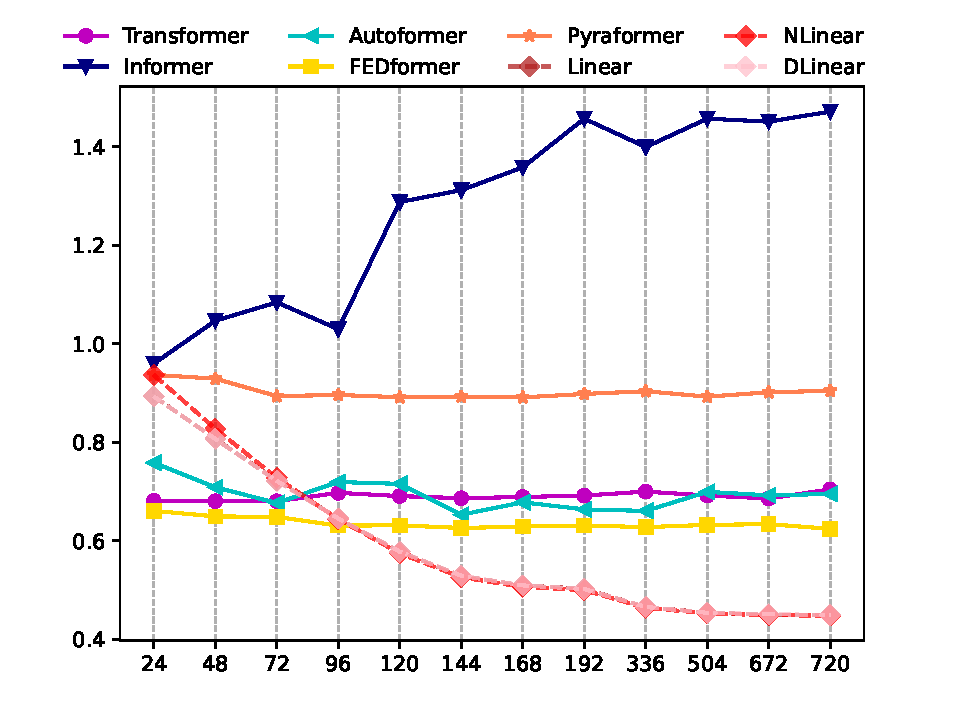
\includegraphics[scale=0.3]{img/traffic_720.pdf}
		\end{minipage}
	}
    \hspace{0.6cm}
	\subfigure[\textbf{720} steps-\textbf{Electricity}]
	{
		\begin{minipage}{3.5cm}
			\centering     
			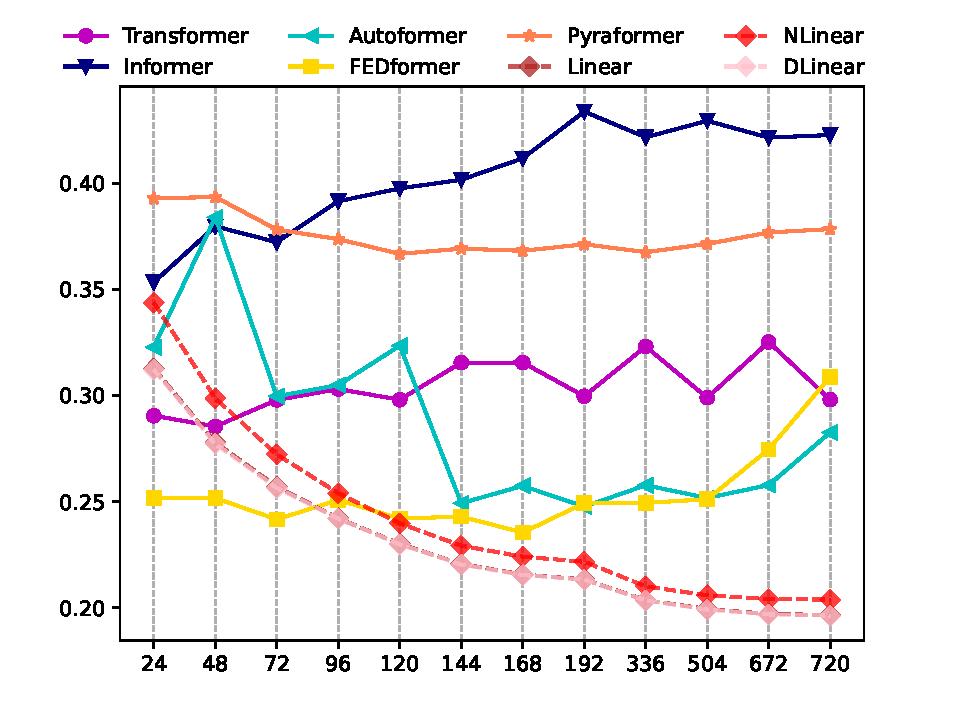
\includegraphics[scale=0.3]{img/electricity_720.pdf} 
		\end{minipage}
	}
    \vspace{-0.2cm}
	\caption{The MSE results (Y-axis) of models with different look-back window sizes (X-axis) of long-term forecasting (T=\textbf{720}) on the Traffic and Electricity datasets. } 
	\label{fig:lookBackWindows}  %图片引用标记
\vspace{-0.2cm}
\end{figure}

\textbf{\emph{What can be learned for long-term forecasting?}}
While the temporal dynamics in the look-back window significantly impact the forecasting accuracy of short-term time series forecasting, we hypothesize that long-term forecasting depends on whether \emph{models can capture the trend and periodicity well only.} That is, the farther the forecasting horizon, the less impact the look-back window itself has.  
%
\begin{table}[h]
\centering
\scalebox{0.9}{
\begin{tabular}{c|cc|cc}
\hline
      \multicolumn{1}{c|}{Methods} &\multicolumn{2}{c|}{FEDformer} & \multicolumn{2}{c}{Autoformer}   \\ \hline
        Input & \emph{Close} & \emph{Far} & \emph{Close} & \emph{Far}  \\ \hline
        Electricity  
        & 0.251 & 0.265 & 0.255 & 0.287  \\
        Traffic 
       & 0.631 & 0.645 & 0.677 & 0.675  \\\hline
        
\end{tabular}
}
\vspace{-0.2cm}
\caption{Comparison of different input sequences under the MSE metric to explore what LTSF-Transformers depend on. If the input is \emph{Close}, we use the $96_{th},..., 191_{th}$ time steps as the input sequence. If the input is \emph{Far}, we use the $0_{th},..., 95_{th}$ time steps. Both of them forecast the $192_{th},...,(192+720)_{th}$ time steps. }
\label{tab:Prior}
\vspace{-0.4cm}
\end{table}

To validate the above hypothesis, in Table~\ref{tab:Prior}, we compare the forecasting accuracy for the same future 720 time steps with data from two different look-back windows: (i). the original input L=96 setting (called \emph{Close}) and (ii). the far input L=96 setting (called \emph{Far}) that is before the original 96 time steps. From the experimental results, the performance of the SOTA Transformers drops slightly, indicating these models only capture similar temporal information from the adjacent time series sequence. Since capturing the intrinsic characteristics of the dataset generally does not require a large number of parameters, i,e. one parameter can represent the periodicity. Using too many parameters will even cause overfitting, which partially explains why \modelname performs better than Transformer-based methods. 



\textbf{\emph{Are the self-attention scheme effective for LTSF?}}
We verify whether these complex designs in the existing Transformer (e.g., Informer) are essential. In Table \ref{tab:Attention}, we gradually transform Informer to Linear. First, we replace each self-attention layer by a linear layer, called \emph{Att.-Linear}, since a self-attention layer can be regarded as a fully-connected layer where weights are dynamically changed.
%Since cross-attention cannot be replaced, we discard the decoder of Informer. Therefore, Att.-Linear is the encoder of Informer, where each self-attention layer is replaced by a linear layer. 
Furthermore, we discard other auxiliary designs (e.g., FFN) in Informer to leave embedding layers and linear layers, named \emph{Embed + Linear}. Finally, we simplify the model to one linear layer. Surprisingly, the performance of Informer grows with the gradual simplification, indicating the unnecessary of the self-attention scheme and other complex modules at least for existing LTSF benchmarks. 


\begin{table}[h]
\centering
%\scriptsize
\scalebox{0.85}{
\begin{tabular}{c|c|cccc}
\hline
        \multicolumn{2}{c|}{Methods} & Informer & \emph{Att.-Linear} & \emph{Embed + Linear} & Linear  \\ \hline
        \multirow{4}{*}{\rotatebox{90}{Exchange}} 
        & 96 & 0.847 & 1.003 & 0.173 & 0.084  \\ 
        & 192 & 1.204 & 0.979 & 0.443 & 0.155  \\ 
        & 336 & 1.672 & 1.498 & 1.288 & 0.301  \\ 
        & 720 & 2.478 & 2.102 & 2.026 & 0.763  \\ \hline
        \multirow{4}{*}{\rotatebox{90}{ETTh1}} 
        & 96 & 0.865 & 0.613 & 0.454 & 0.400  \\ 
        & 192 & 1.008 & 0.759 & 0.686 & 0.438  \\ 
        & 336 & 1.107 & 0.921 & 0.821 & 0.479  \\ 
        & 720 & 1.181 & 0.902 & 1.051 & 0.515 \\ \hline
    \end{tabular}
}
\vspace{-0.2cm}
\caption{The MSE comparisons of gradually transforming Informer to a Linear from the left to right columns. \emph{Att.-Linear} is a structure that replaces each attention layer with a linear layer. \emph{Embed + Linear} is to drop other designs and only keeps embedding layers and a linear layer. The look-back window size is 96.}
\label{tab:Attention}
\vspace{-0.3cm}
\end{table}
%Shuffle after embedding

\begin{table*}[h]
\centering
\scalebox{0.85}{
\begin{tabular}{c|c|ccc|ccc|ccc|ccc}
\hline
\multicolumn{2}{c|}{Methods} & \multicolumn{3}{c|}{Linear} &\multicolumn{3}{c|}{FEDformer} & \multicolumn{3}{c|}{Autoformer} & \multicolumn{3}{c}{Informer} \\ \hline
\multicolumn{2}{c|}{Predict Length} & \emph{Ori.} & \emph{Shuf.} & \emph{Half-Ex.} & \emph{Ori.} & \emph{Shuf.} & \emph{Half-Ex.} & \emph{Ori.} & \emph{Shuf.} & \emph{Half-Ex.} & \emph{Ori.} & \emph{Shuf.} & \emph{Half-Ex.} \\ \hline
        \multirow{4}{*}{\rotatebox{90}{Exchange}}
        &96 & 0.080 & 0.133 & 0.169 & 0.161 & 0.160 & 0.162 & 0.152 & 0.158 & 0.160 & 0.952 & 1.004 & 0.959  \\ 
        &192 & 0.162 & 0.208 & 0.243 & 0.274 & 0.275 & 0.275 & 0.278 & 0.271 & 0.277 & 1.012 & 1.023 & 1.014 \\ 
        &336 & 0.286 & 0.320 & 0.345 & 0.439 & 0.439 & 0.439 & 0.435 & 0.430 & 0.435 & 1.177 & 1.181 & 1.177  \\ 
        &720 & 0.806 & 0.819 & 0.836 & 1.122 & 1.122 & 1.122 & 1.113 & 1.113 & 1.113 & 1.198 & 1.210 & 1.196  \\ \hline
        &Average Drop & N/A & 27.26\% & 46.81\% & N/A & -0.09\% & 0.20\% & N/A & 0.09\% & 1.12\% & N/A & -0.12\% & -0.18\%\\ \hline
        \multirow{4}{*}{\rotatebox{90}{ETTh1}}
        &96 & 0.395 & 0.824 & 0.431 & 0.376 & 0.753 & 0.405 & 0.455 & 0.838 & 0.458 & 0.974 & 0.971 & 0.971   \\ 
        &192 & 0.447 & 0.824 & 0.471 & 0.419 & 0.730 & 0.436 & 0.486 & 0.774 & 0.491 & 1.233 & 1.232 & 1.231   \\ 
        &336 & 0.490 & 0.825 & 0.505 & 0.447 & 0.736 & 0.453 & 0.496 & 0.752 & 0.497 & 1.693 & 1.693 & 1.691 \\ 
        &720 & 0.520 & 0.846 & 0.528 & 0.468 & 0.720 & 0.470 & 0.525 & 0.696 & 0.524 & 2.720 & 2.716 & 2.715  \\ \hline
        &Average Drop & N/A & 81.06\% & 4.78\% & N/A & 73.28\% & 3.44\% & N/A & 56.91\% & 0.46\% & N/A & 1.98\% & 0.18\%  \\ \hline
\end{tabular}
}
\vspace{-0.2cm}
\caption{The MSE comparisons of models when shuffling the raw input sequence. \emph{Shuf.} randomly shuffles the input sequence. \emph{Half-EX.} randomly exchanges the first half of the input sequences with the second half. Average Drop is the average performance drop under all forecasting lengths after shuffling. All results are the average test MSE of five runs.}
\label{tab:Shuffle}
\vspace{-0.4cm}
\end{table*}

\textbf{\emph{Can existing LTSF-Transformers preserve temporal order well?}}
Self-attention is inherently permutation-invariant, i.e., regardless of the order. However, in time-series forecasting, the sequence order often plays a crucial role. We argue that even with positional and temporal embeddings, existing Transformer-based methods still suffer from temporal information loss. In Table ~\ref{tab:Shuffle}, we shuffle the raw input before the embedding strategies. Two shuffling strategies are presented: \emph{Shuf.} randomly shuffles the whole input sequences and \emph{Half-Ex.} exchanges the first half of the input sequence with the second half.
%
Interestingly, compared with the original setting (\emph{Ori.}) on the Exchange Rate, the performance of all Transformer-based methods does not fluctuate even when the input sequence is randomly shuffled. By contrary, the performance of \modelname is damaged significantly. These indicate that LTSF-Transformers with different positional and temporal embeddings preserve quite limited temporal relations and are prone to overfit on noisy financial data, while the \modelname can model the order naturally and avoid overfitting with fewer parameters. 
%

For the ETTh1 dataset, FEDformer and Autoformer introduce time series inductive bias into their models, making them can extract certain temporal information when the dataset has more clear temporal patterns (e.g., periodicity) than the Exchange Rate. Therefore, the average drops of the two Transformers are 73.28\% and 56.91\% under the \emph{Shuf.} setting, where it loses the whole order information. Moreover, Informer still suffers less from both \emph{Shuf.} and \emph{Half-Ex.} settings due to its no such temporal inductive bias. Overall, the average drops of \modelname are larger than Transformer-based methods for all cases, indicating the existing Transformers do not preserve temporal order well.
%Although FEDformer shows a comparable performance drop, we point out that it uses no self-attention layer but one cross-attention layer in its architecture.  


%

\begin{table}[h]
    \centering
    % \scriptsize
    \scalebox{0.85}
    {
            \begin{tabular}{c|c|cccc}
            \hline
            \multirow{2}{*}{Methods}    & \multirow{2}{*}{Embedding}                & \multicolumn{4}{c}{Traffic}                                   \\
                                         &                            & 96             & 192            & 336            & 720            \\\hline \hline
            \multirow{4}{*}{FEDformer}   & All                       & 0.597          & 0.606          & 0.627          & 0.649          \\
                                         & wo/Pos.                   & \textbf{0.587} & \textbf{0.604} & \textbf{0.621} & \textbf{0.626} \\
                                         & wo/Temp.                  & 0.613          & 0.623          & 0.650          & 0.677          \\
                                         & wo/Pos.-Temp.             & 0.613          & 0.622          & 0.648          & 0.663          \\\hline\hline
            \multirow{4}{*}{Autoformer}  & All              & 0.629          & 0.647          & 0.676          & \textbf{0.638} \\
                                         & wo/Pos.          & \textbf{0.613} & \textbf{0.616} & \textbf{0.622} & 0.660          \\
                                         & wo/Temp.         & 0.681          & 0.665          & 0.908          & 0.769          \\
                                         & wo/Pos.-Temp.    & 0.672          & 0.811          & 1.133          & 1.300          \\\hline\hline
            \multirow{4}{*}{Informer}    & All              & \textbf{0.719} & \textbf{0.696} & \textbf{0.777} & \textbf{0.864}          \\
                                         & wo/Pos.          & 1.035          & 1.186          & 1.307          & 1.472          \\
                                         & wo/Temp.         & 0.754          & 0.780          & 0.903          & 1.259 \\
                                         & wo/Pos.-Temp.    & 1.038          & 1.351          & 1.491          & 1.512         
             \\\hline
            \end{tabular}
            }
            \vspace{-0.3cm}
            \caption{The MSE comparisons of different embedding strategies on Transformer-based methods with look-back window size $96$ and forecasting lengths $\{96,192,336,720\}$. }
\label{tab:embedding}
\vspace{-0.5cm}
\end{table}      
            
            

\textbf{\emph{How effective are different embedding strategies?}}
%
We study the benefits of position and timestamp embeddings used in Transformer-based methods. 
%Existing works mainly use three types of embeddings, i.e., a fixed positional embedding used in Vanilla Transformer (Pos.), a learnable timestamp embedding (Temp.), and a necessary channel projection embedding.
%
In Table~\ref{tab:embedding}, the forecasting errors of Informer largely increase without positional embeddings (wo/Pos.). Without timestamp embeddings (wo/Temp.) will gradually damage the performance of Informer as the forecasting lengths increase. 
%
Since Informer uses a single time step for each token, it is necessary to introduce temporal information in tokens.

%
Rather than using a single time step in each token, FEDformer and Autoformer input a sequence of timestamps to embed the temporal information. 
%
Hence, they can achieve comparable or even better performance without fixed positional embeddings. However, without timestamp embeddings, the performance of Autoformer declines rapidly because of the loss of global temporal information. Instead, thanks to the frequency-enhanced module proposed in FEDformer to introduce temporal inductive bias, it suffers less from removing any position/timestamp embeddings. 
%



\textbf{\emph{Is training data size a limiting factor for existing LTSF-Transformers?}}
Some may argue that the poor performance of Transformer-based solutions is due to the small sizes of the benchmark datasets. 
%As Transformers can achieve significant results in NLP and CV areas, where they have large-scale data for training. 
Unlike computer vision or natural language processing tasks, TSF is performed on collected time series, and it is difficult to scale up the training data size. In fact, the size of the training data would indeed have a significant impact on the model performance. Accordingly, we conduct experiments on Traffic, comparing the performance of the model trained on a full dataset (17,544*0.7 hours), named \emph{Ori.}, with that trained on a shortened dataset (8,760 hours, i.e., 1 year), called \emph{Short}. Unexpectedly, Table~\ref{tab:shortenTraffic} presents that the prediction errors with reduced training data are lower in most cases. This might because the whole-year data maintains more clear temporal features than a longer but incomplete data size. While we cannot conclude that we should use less data for training, it demonstrates that the training data scale is not the limiting reason for the performances of Autoformer and FEDformer. 

\begin{table}[h]
\centering
\scalebox{0.9}{
\begin{tabular}{c|cc|cc}
\hline
Methods        & \multicolumn{2}{c|}{FEDformer}     & \multicolumn{2}{c}{Autoformer}    \\ \hline
Dataset& \emph{Ori.} & \emph{Short} & \emph{Ori.} & \emph{Short}  \\\hline
96                  &0.587 & \textbf{0.568} &0.613 & \textbf{0.594} \\
192                  &0.604 & \textbf{0.584} &\textbf{0.616} & 0.621 \\
336                  &0.621 & \textbf{0.601} &0.622 & \textbf{0.621} \\
720                   &0.626 & \textbf{0.608} &0.660 & \textbf{0.650} \\ \hline
\end{tabular}
}
\vspace{-0.2cm}
\caption{The MSE comparison of two training data sizes.}
\vspace{-0.3cm}
\label{tab:shortenTraffic}
\end{table}


\textbf{\emph{Is efficiency really a top-level priority?}}
% \TODO{[ADD a Table here]: flops}
Existing LTSF-Transformers claim that the $O\left(L^{2}\right)$ complexity of the vanilla Transformer is unaffordable for the LTSF problem. Although they prove to be able to improve the theoretical time and memory complexity from $O\left(L^{2}\right)$ to $O\left(L\right)$, it is unclear whether \emph{1) the actual inference time and memory cost on devices are improved, and 2) the memory issue is unacceptable and urgent for today's GPU (e.g., an NVIDIA Titan XP here).}
%
In Table ~\ref{tab:efficiency}, we compare the average practical efficiencies with 5 runs. Interestingly, compared with the vanilla Transformer (with the same DMS decoder), most Transformer variants incur similar or even worse inference time and parameters in practice. These follow-ups introduce more additional design elements to make practical costs high. Moreover, the memory cost of the vanilla Transformer is practically acceptable, even for output length $L=720$, which weakens the importance of developing a memory-efficient Transformers, at least for existing benchmarks. 


\begin{table}[h]
\vspace{-0.1cm}
        \centering
        \scalebox{0.9}
        % \scriptsize
        {
        	{%
                \begin{tabular}{c|cccc} \hline
                Method      & MACs & Parameter & Time & Memory\\\hline
                DLinear  & \textbf{0.04G}   & \textbf{139.7K}    & \textbf{0.4ms}     &\textbf{687MiB}        \\\hline
                Transformer$\times$ & 4.03G   & 13.61M     & 26.8ms     &6091MiB \\
                Informer    & 3.93G   & 14.39M     & 49.3ms     &3869MiB        \\
                Autoformer  & 4.41G   & 14.91M     & 164.1ms     &7607MiB        \\
                Pyraformer & 0.80G    &  241.4M$^*$   & 3.4ms     &7017MiB          \\
                FEDformer   & 4.41G   & 20.68M     & 40.5ms     &4143MiB \\\hline       
                % GBRT        &   -         &    -        & 30.7ms    & -              & - & - & L  \\
                % ARIMA       &     -       &     -       & 787.5ms    & -              & - & - & L\\          
                \end{tabular}%
        	}
            }
            \begin{tablenotes}
            \tiny
            {
            \item - $\times$ is modified into the same one-step decoder, which is implemented in the source code from Autoformer.
            \item - $*$ 236.7M parameters of Pyraformer come from its linear decoder. 
            }
            \end{tablenotes} %添加此处
            \vspace{-0.2cm}
        \caption{Comparison of practical efficiency of LTSF-Transformers under L=96 and T=720 on the Electricity. MACs are the number of multiply-accumulate operations. We use Dlinear for comparison since it has the double cost in \modelname. The inference time averages 5 runs.}
\label{tab:efficiency}
\vspace{-0.3cm}
\end{table}




